% This is "sig-alternate.tex" V2.0 May 2012
% This file should be compiled with V2.5 of "sig-alternate.cls" May 2012
%
% This example file demonstrates the use of the 'sig-alternate.cls'
% V2.5 LaTeX2e document class file. It is for those submitting
% articles to ACM Conference Proceedings WHO DO NOT WISH TO
% STRICTLY ADHERE TO THE SIGS (PUBS-BOARD-ENDORSED) STYLE.
% The 'sig-alternate.cls' file will produce a similar-looking,
% albeit, 'tighter' paper resulting in, invariably, fewer pages.
%
% ----------------------------------------------------------------------------------------------------------------
% This .tex file (and associated .cls V2.5) produces:
%       1) The Permission Statement
%       2) The Conference (location) Info information
%       3) The Copyright Line with ACM data
%       4) NO page numbers
%
% as against the acm_proc_article-sp.cls file which
% DOES NOT produce 1) thru' 3) above.
%
% Using 'sig-alternate.cls' you have control, however, from within
% the source .tex file, over both the CopyrightYear
% (defaulted to 200X) and the ACM Copyright Data
% (defaulted to X-XXXXX-XX-X/XX/XX).
% e.g.
% \CopyrightYear{2007} will cause 2007 to appear in the copyright line.
% \crdata{0-12345-67-8/90/12} will cause 0-12345-67-8/90/12 to appear in the copyright line.
%
% ---------------------------------------------------------------------------------------------------------------
% This .tex source is an example which *does* use
% the .bib file (from which the .bbl file % is produced).
% REMEMBER HOWEVER: After having produced the .bbl file,
% and prior to final submission, you *NEED* to 'insert'
% your .bbl file into your source .tex file so as to provide
% ONE 'self-contained' source file.
%
% ================= IF YOU HAVE QUESTIONS =======================
% Questions regarding the SIGS styles, SIGS policies and
% procedures, Conferences etc. should be sent to
% Adrienne Griscti (griscti@acm.org)
%
% Technical questions _only_ to
% Gerald Murray (murray@hq.acm.org)
% ===============================================================
%
% For tracking purposes - this is V2.0 - May 2012

\documentclass{sig-alternate}
\usepackage[utf8]{inputenc}
\usepackage{algorithmic}
\usepackage{algorithm}
\usepackage{multirow}

\begin{document}
%
% --- Author Metadata here ---
%\conferenceinfo{WOODSTOCK}{'97 El Paso, Texas USA}
%\CopyrightYear{2007} % Allows default copyright year (20XX) to be over-ridden - IF NEED BE.
%\crdata{0-12345-67-8/90/01}  % Allows default copyright data (0-89791-88-6/97/05) to be over-ridden - IF NEED BE.
% --- End of Author Metadata ---

\title{Using Collective Matrix Factorization and Tags to improve a Recommender System}
%
% You need the command \numberofauthors to handle the 'placement
% and alignment' of the authors beneath the title.
%
% For aesthetic reasons, we recommend 'three authors at a time'
% i.e. three 'name/affiliation blocks' be placed beneath the title.
%
% NOTE: You are NOT restricted in how many 'rows' of
% "name/affiliations" may appear. We just ask that you restrict
% the number of 'columns' to three.
%
% Because of the available 'opening page real-estate'
% we ask you to refrain from putting more than six authors
% (two rows with three columns) beneath the article title.
% More than six makes the first-page appear very cluttered indeed.
%
% Use the \alignauthor commands to handle the names
% and affiliations for an 'aesthetic maximum' of six authors.
% Add names, affiliations, addresses for
% the seventh etc. author(s) as the argument for the
% \additionalauthors command.
% These 'additional authors' will be output/set for you
% without further effort on your part as the last section in
% the body of your article BEFORE References or any Appendices.

\numberofauthors{1} %  in this sample file, there are a *total*
% of EIGHT authors. SIX appear on the 'first-page' (for formatting
% reasons) and the remaining two appear in the \additionalauthors section.
%
\author{
% You can go ahead and credit any number of authors here,
% e.g. one 'row of three' or two rows (consisting of one row of three
% and a second row of one, two or three).
%
% The command \alignauthor (no curly braces needed) should
% precede each author name, affiliation/snail-mail address and
% e-mail address. Additionally, tag each line of
% affiliation/address with \affaddr, and tag the
% e-mail address with \email.
%
% 1st. author
Cristopher Arenas\\
\affaddr{Universidad Técnica Federico Santa María}\\
\affaddr{Vicuña Mackenna 3939}\\
\affaddr{Santiago, Chile}\\
\email{cristopher.arenas@alumnos.usm.cl}\\
}

\maketitle
\begin{abstract}
In many recommender systems, there are not enough information to realize good predictions, mostly because poor information from data sources are used. Users rate few items in the dataset. This paper presents a improvement to recommender systems using Collective Matrix Factorization and tag information. A existing work will be used and some aditional contributions will be exposed. 
\end{abstract}

% A category with the (minimum) three required fields
%\category{H.4}{Information Systems Applications}{Miscellaneous}
%A category including the fourth, optional field follows...
%\category{D.2.8}{Software Engineering}{Metrics}[complexity measures, performance measures]

%\terms{Theory}

\keywords{matrix factorization, tags, gradient descent method}

\section{Introduction}

Recommender Systems are used to provide recommendation to users about items that they could like. The re-commendation problem consist to predict for an user $u$ the preference about an item $i$, tipically with a range of values $r$ called rating. 

Different approaches to resolve the problem have been proposed. There are methods based in Collaborative Filtering (CF) \cite{schafer2007collaborative} that started with the works about this topic. CF can be based in items \cite{sarwar2001item}, users \cite{herlocker1999algorithmic} or ratings \cite{lemire2005slope}. This approach find similar entities to the user and propose a list with items of new items for that user. This items could be novelty and interesting for that user. 

A common issue that will be considered is the problem of sparity in CF. The information of the datasets used in this cases shows that the most part of the users rate a low quantity of items. A litte quantity of users rate a considerably amount of items and the rest of them rate extremly few items. This produces problems to generate predictions in ratings because there are not enough information available.

Other approaches based in matrix factorizations \cite{koren2009matrix} try to solve the sparsity problem using filling techniques in a matrix that conects users and items. The predicted value will be considered as a product of two vectors and will be represented in a matrix \textit{user-item}.

This work will use an approach called Collective Matrix Factorization and will consider extra information derived from tags. A tag is commonly a label asigned by users to anitem that share a feature with others.

The paper is organized as follows. Section 2 present the matrix factorization used in recommender systems. Section 3 shows the method used in this work and aditional considerations used. Section 4 explains the experiments realized and section 5 shows the results obtained. Finally, section 6 shows the conclusions of this work.

\section{Related Work}

The matrix factorization approaches \cite{koren2009matrix} consider the factorization of a matrix $U$ that relates users an items. A cell value of this matrix represent the rating that an user $u$ assign to an item $i$. Traditional approaches try to minimize the error function:

\begin{equation}
E = \sum_{(u,i)\in K} (r_{ui}-q_i^Tp_{u})^2 + \lambda(||q_i||^2+||p_u||^2)
\end{equation}

Where $r_{ui}$ is the rating of the user $u$ for the item $i$ and the vector product $q_i^Tp_u$ determine an aproximate rating for the previous pair. $\lambda$ is used to avoid overfitting.

There are similar aproaches that adds bias terms to the error function, and others consider aditional imput sources. 

\section{Proposed Method}

The base of this work is presented in \cite{tag}. There are three matrices that relates $m$ users, $n$ items and $p$ tags:
\begin{itemize}
\item $U(u,i)$: user-item matrix. Shows the \textit{rating} of user $u$ for an item $i$.
\item $T(u,t)$: user-tag matrix. Shows the \textit{preference} of an user $u$ for the tag $t$.
\item $G(i,t)$: tag-item matrix. Shows \textit{relevance} between item $i$ and tag $t$.
\end{itemize}

The $U$ matrix is constructed with traditional approaches of matrix factorization. $G$ matrix is constructed in a similar way to $U$ matrix, considering tags in place of items. $T$ matrix is constructed using the other two matrices. The equation \eqref{eq:t} shows how to determine the relation between the user $u$ and tag $t$.

\begin{equation}
\label{eq:t}
T(u,t) = \frac{1}{N} \sum_{k=1}^{n}U(u,k) \times G(k,t)
\end{equation}

$N$ is a normalized factor that consider the number of $k$ that $U(u,k)$ and $G(k,t)$ are not zero.

The next step is construct two matrices $U'$ and $T'$ using users, items, tags and latent factors.
\begin{equation}
\label{eq:u}
U' = XY^T
\end{equation} 

\begin{equation}
\label{eq:u}
T' = XZ^T
\end{equation} 

Where $X$, $Y$ and $Z$ are submatrices. $X$ is the relation between users and latent factors, $Y$ is the relation between items and latent factors and $Z$ is the relation between tags and latent factors.

Later, the Gradient Descent Method (GDM) is performed to minimize the error between the real values ($U$ and $T$) and the aproximated values ($U'$ and $T')$. The error function to minimize is showed in \eqref{eq:error}.

\begin{equation}
\label{eq:error}
\begin{aligned}
ER(X,Y,Z) &= \frac{1}{2}||J \circ (U-XY^T)||^{2}_{F}+\frac{\alpha}{2}||T-XZ^T||^{2}_{F}\\
&+\frac{\beta}{2}\left( ||X||^{2}_{F} + ||Y||^{2}_{F} + ||Z||^{2}_{F} \right)
\end{aligned}
\end{equation}

$J$ is an Indicator Matrix where $J(a,b)=1$ if an user $a$ has rated the item $b$ and zero in other case. The GDM moves the values of the matrices $X$, $Y$ and $Z$ in direction of gradients $\nabla_XER$, $\nabla_YER$ and $\nabla_ZER$.

\begin{equation}
\label{eq:gradientx}
\nabla_XER = \left[ J \circ (XY^T-U) \right] Y + \alpha (XZ^T-T)Z + \beta X
\end{equation}
\begin{equation}
\label{eq:gradienty}
\nabla_YER = \left[ J \circ (XY^T-U) \right] X + \beta Y
\end{equation}
\begin{equation}
\label{eq:gradientz}
\nabla_ZER = \alpha (XZ^T-T)X + \beta Z
\end{equation}

The GDM starts with random values in range (0,1) for $X$, $Y$ and $Z$. Later, calculates a step $\gamma$ to move this matrices in direction of the gradient. Finally, a value $U'=XY^T$ is returned and contain values that $U$ matrix does not have. This new values correspond to predicted values to the user $u$ rating the item $i$. The Algorithm \ref{alg:gdm} summarizes the GDM.

\begin{algorithm}
\caption{Gradient Descent Method. Adapted from \cite{tag}}
\label{alg:gdm}
\begin{algorithmic}[1]
\STATE Initialize $X$, $Y$, $Z$ with random number in range (0,1)
\STATE $t = 0$
\WHILE{$t < max\_iteration$}
\STATE Get gradients $\nabla_XER$, $\nabla_YER$ and $\nabla_ZER$.
\STATE $\gamma=1$
\WHILE{$(ER(X_t-\gamma\nabla_{X_t},Y_t-\gamma\nabla_{Y_t},Z_t-\gamma\nabla_{Z_t})>ER(X_t,Y_t,Z_t))$}
\STATE $\gamma = \gamma/2$
\ENDWHILE
\STATE $X_{t+1} = X_{t}-\gamma\nabla_{X_t}$
\STATE $Y_{t+1} = Y_{t}-\gamma\nabla_{Y_t}$
\STATE $Z_{t+1} = Z_{t}-\gamma\nabla_{Z_t}$
\STATE $t = t+1$
\ENDWHILE
\end{algorithmic}
\end{algorithm}

\section{Experiments}

The are two cases that \cite{tag} took for $\alpha$ and $\beta$. First, the baseline consider $\alpha=0$ and $\beta=1$. This case correspond to traditional matrix factorization approach, using only users and items. Later, the case $\alpha=1$ and $\beta=1$ was consider the best case that use tag information.

The dataset from MovieLens was considered to realize experiments. This dataset is composed by 1,000,209 ratings of 3,682 movies made by 6,040 users. Also, data from Tag-Genome, in the MovieLens site, was used for consider information about tags. Tag-Genome is composed by 9,734 movies and 1,128 tags. The total quantity of movies considered were those who was present in ratings and tags dataset simultaneously. This means that only 3,642 movies were considered to realize the experiments.

There were three experiments realized. First, a comparation about using different number of latent factors was considered. Later, a prediction of ratings were determinated using GDM with the minimization of the error function \eqref{eq:error} MAE and RMSE metrics were considered to compare the use of tags and the traditional approach. Finally, a Top-N ranking was generated for users and average of nDCG metric was calculated.

The data was split into training and test. 80\% of the data was used as training set and the other 20\% was used as test set. The idea of prediction and Top-N ranking was predict the values of the test set using the training set to generate the matrices and execute the GDM.

\section{Results}

The Figure \ref{fig:error} shows the error function using 1, 3 and 10 latent factors. The GDM was executed for 100 iterations and only the case $\alpha=1$ and $\beta=1$ was considered.

\begin{figure}[!htb]
\centering
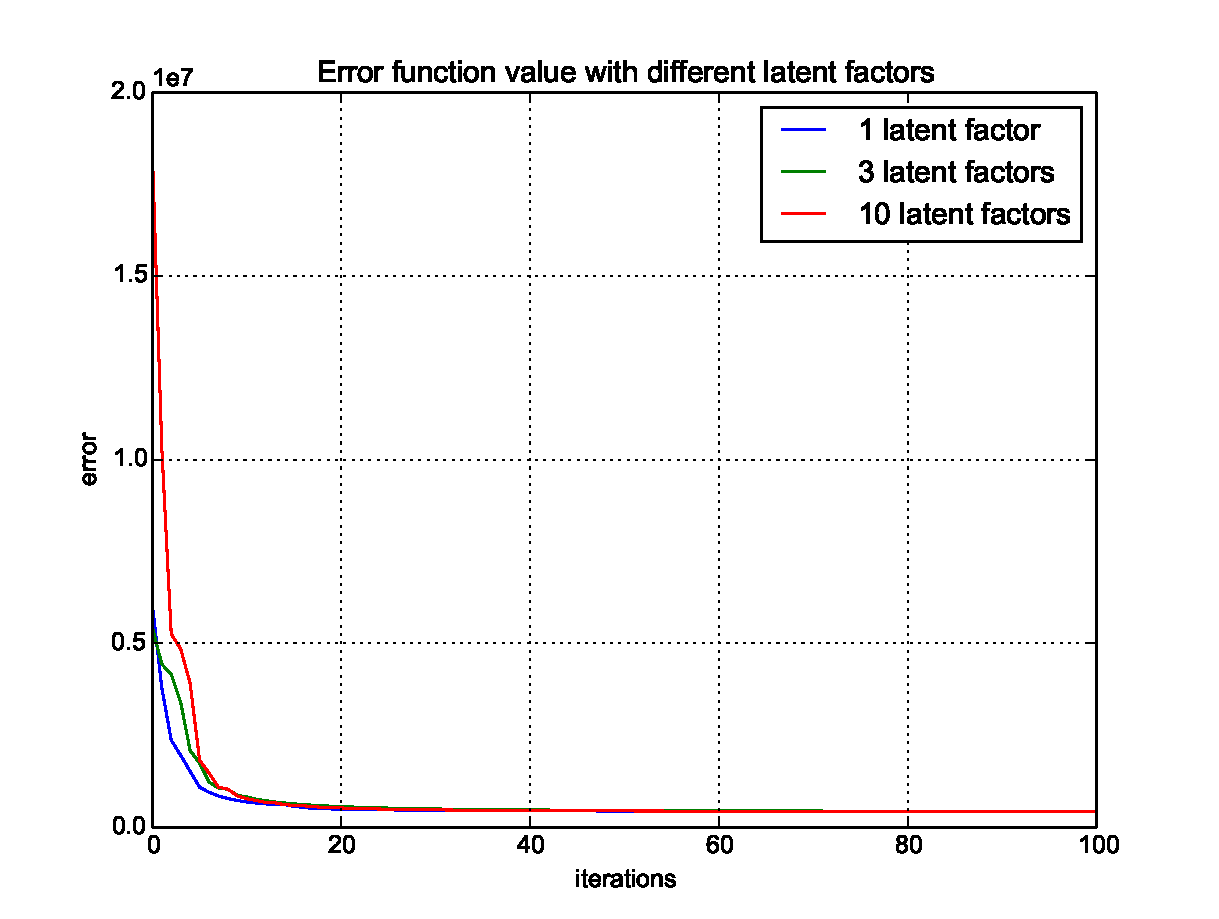
\includegraphics[width=0.5\textwidth]{exp1}
\caption{Error function using three different latent factors.}
\label{fig:error}
\end{figure}

The Figure \ref{eq:error} shows that in the first moments of the algorithm the error value is high and in the next 10 iterations this value decreases faster. Since iteration 40, the error decreases slowly. Using more latent factors cause more error in the begining of the algorithm. There are not a big difference in the value of the error in the last iterations.  

The Table \ref{tab:metric1} shows the results for the metrics MAE and RMSE for the two scenarios (with tags consider $\alpha=1$ and $\beta=1$ and without tags consider $\alpha=0$ and $\beta=1$). In both cases, GDM was excecuted with 200 iterations.

\begin{table*}[!htb]
\caption{MAE and RMSE considering two scenarios.}
\centering
\begin{tabular}{|c|c|c|}
\hline
Metric & With tags & Without tags\\ \hline \hline
$MAE$ & 0.7236 & 0.6961\\ \hline
$RMSE$ & 0.9264 & 0.8945\\
\hline
\end{tabular}
\label{tab:metric1}
\end{table*}

\begin{table*}
\centering
\caption{nDCG@p metric for two scenarios and differents values of p}
\begin{tabular}{|c|c|c|c|c|c|c|}
\hline
\multirow{2}{*}{$p$} & \multicolumn{2}{|c|}{Best user} & \multicolumn{2}{|c|}{Worst user} & \multicolumn{2}{|c|}{Average} \\ \cline{2-7}
 & With tags & Without tags & With tags & Without tags & With tags & Without tags \\ \hline \hline
1 & 0.7869 & 0.8354 & 0.7869 & 0.8354 & 0.7869 & 0.8354 \\ \hline
3 & 0.7855 & 0.8323 & 0.6431 & 0.6581 & 0.7169 & 0.7337\\ \hline
5 & 0.7811 & 0.8256 & 0.4256 & 0.5164 & 0.6353 & 0.6740\\ \hline
10 & 0.9966 & 0.8666 & 0.4147 & 0.5002 & 0.6888 & 0.7157\\ \hline
20 & 0.9676 & 0.9658 & 0.3974 & 0.4682 & 0.6798 & 0.7066\\ \hline
\end{tabular}
\label{tab:ndcg}
\end{table*}

The values obtained shows that there are not enough difference between use tags or not. The best values of MAE and RMSE are those who were determinated without use tags.

The Table \ref{tab:ndcg} shows the values obtained for the $nDCG@p$ metric. Different values of $p$ were used. The worst user, best user and average of this metric was calculated. The values shows that mostly of the cases are better when tags are not considered. In some cases ($p=10$ and $p=20$), the best user delivered a better value for nDCG when tags were takes into account.

\section{Conclusions}
There are different ways to do a matrix factorization to determine a prediction rating for users and items. In this work a method defined in a previous work was realized and aditional metrics and analisys were showed. 

The purpouse of this work was show that using tags in a collective matrix factorization could be better than realize a simple matrix factorization. Considering the results obtained, there is not possible to conclude this proposition. The values of the metrics used where very similar considering the use of the tag information and only information of the traditional approach. Probably, this unespected results were obtained because the $T$ matrix constructed was not completly full of values, and this factor impacted in lower performance. When more latent factors were used, initially were obtained worst values in the error function, but in the last iterations there will be not a significant difference between them.  

Future work includes realize a more exaustive revision of other metrics and dataset used. The generation of the matrices will be an issue that will be necessary to review.
\bibliographystyle{abbrv}
\bibliography{sigproc}


\end{document}
